% Courbes de niveau de S(b) = S(b̂) + (b-b̂)'X'X(b-b̂). La forme des ellipses est
% celle de X'X ; leur allongement mesure le mauvais conditionnement.
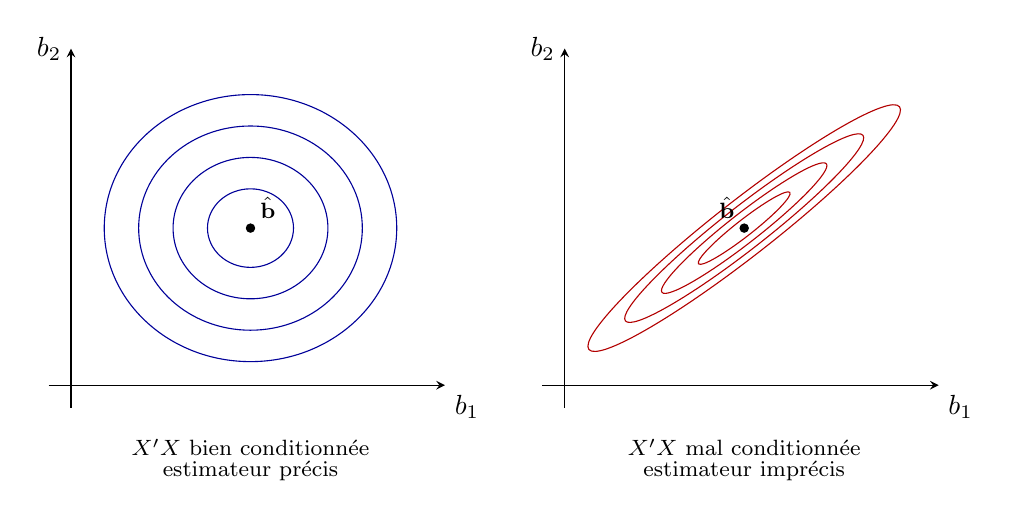
\begin{tikzpicture}[>=stealth, scale=0.95]

\begin{scope}
  \draw[->] (-0.3,0) -- (5.0,0) node[below right] {$b_1$};
  \draw[->] (0,-0.3) -- (0,4.5) node[left] {$b_2$};
  \foreach \r in {0.5,0.9,1.3,1.7}
    \draw[blue!60!black] (2.4,2.1) ellipse [x radius=\r*1.15, y radius=\r*1.05];
  \fill (2.4,2.1) circle (1.8pt) node[above right, font=\footnotesize] {$\hat{\mathbf b}$};
  \node[font=\footnotesize, align=center] at (2.4,-1.0)
       {$X'X$ bien conditionnée\\[-2pt] estimateur précis};
\end{scope}

\begin{scope}[xshift=6.6cm]
  \draw[->] (-0.3,0) -- (5.0,0) node[below right] {$b_1$};
  \draw[->] (0,-0.3) -- (0,4.5) node[left] {$b_2$};
  \foreach \r in {0.5,0.9,1.3,1.7}
    \draw[red!70!black, rotate around={38:(2.4,2.1)}]
      (2.4,2.1) ellipse [x radius=\r*1.55, y radius=\r*0.22];
  \fill (2.4,2.1) circle (1.8pt) node[above left, font=\footnotesize] {$\hat{\mathbf b}$};
  \node[font=\footnotesize, align=center] at (2.4,-1.0)
       {$X'X$ mal conditionnée\\[-2pt] estimateur imprécis};
\end{scope}

\end{tikzpicture}
